\section{Case Studies}\label{sec:usecases}

In this section, we provide four\xxx case studies demonstrating the practical
utility of heterogeneous FDE not achievable with prior work. We cover a wide
range of situations, highlighting concerns like meeting latency goals, trading
off security and writable space, and keeping within an energy budget, all
demonstrating the utility of both temporal and spatial switching strategies. All
experiments are repeated multiple times.


% ===========================================================
\subsection{Battery Saver Mode}\label{subsec:uc1}

% About: motivation
In this first case study, we revisit the motivational example.  Here, the mobile
device is ``forced'' to locally encrypt files with Freestyle Balanced Cipher
(``\cone'') for safely backing up the file to the backend cloud, but when the
battery saver mode is on, the device will switch to a more energy-efficient
cipher, ChaCha8 (``\ctwo''), and at the same time pausing the backup upload to
the cloud momentarily (\eg the company does not want files to be saved in the
cloud without \cone encryption. Our goal is to complete I/Os as much as we can
before the device dies.

% About: setup
To simulate I/O activity, we begin randomly writing 10 40MB files using the
Freestyle Balanced cipher for 2 minutes.  After the first 5 seconds, the device
enters ``battery saver'' mode, which we simulate by underclocking the cores to
their lowest frequencies and using \texttt{taskset} to transition \sys processes
to the energy-efficient LITTLE cores.  In this low battery mode, \sys switches
to the ChaCha8 cipher.

\hsg{I dont' understand Figure \figref{usecase-battery}. You said after 5
seconds.  we switch to ChaCha8. But why the FB+ChaCha line is still going up?
Why it doesn't flat out like the ChaCha line?? and why do even need to show the
ChaCha8 only line?}

\def \fgh {1in}

\begin{figure}[t]
    \centering
    %{\begin{tikzpicture}[baseline]

    \pgfmathsetmacro{\xmax}{130} % set the maximum x value
    \pgfmathsetmacro{\ymax}{50} % set the maximum y value
    \pgfmathsetmacro{\ymaxbreak}{50.1} % set the y value at which overflow is drawn

    \begin{groupplot}[
        group style={
            group size=1 by 2,
            ylabels at=edge left,
            xlabels at=edge bottom,
            yticklabels at=edge left,
            xticklabels at=edge bottom,
            vertical sep=10pt,
        },
        %axis x line*=bottom,
        height=4cm,
        width=\linewidth,
        tick align=outside,
        tick pos=bottom, % make sure ticks only appear at the bottom and left axes
        tick style={ black },
        y tick label style={ /pgf/number format/fixed, /pgf/number format/precision=0 },
        grid style={ dotted, gray },
        every node near coord/.append style={font=\tiny},
        %
        % % magic to make the numbers appear above the overly long bars:
        % visualization depends on={rawy \as \rawy}, % save original y values
        % restrict y to domain*={ % now clip/restrict any y value to ymax
        %     \pgfkeysvalueof{/pgfplots/ymin}:\ymaxbreak
        % },
        % after end axis/.code={ % draw squiggly line indicating break
        %     \draw [semithick, white, decoration={snake,amplitude=0.1mm,segment length=0.75mm,post length=0.375mm}, decorate] (rel axis cs:0,1.01) -- (rel axis cs:1,1.01);
        % },
        % nodes near coords={\color{.!75!black}\pgfmathprintnumber\rawy}, % print the original y values (darkened in case they are too light)...
        % nodes near coords greater equal only=\ymax, % ... but ONLY if they are >= ymax
        clip=true, % allow clip to protrude beyond ymax if false
        % % Custom stuff to edit per template
        %
        xlabel={Time (s)},
        xlabel near ticks,
        xlabel shift={-4mm},
        xmin=0, xmax=\xmax,
        xtick={ 0, \xmax },
        enlargelimits=false, % add some breathing room along the x axis's sides
        % %major x tick style=transparent,
        %
        ylabel near ticks,
        ylabel shift={-5mm},
        ymajorgrids=true,
        %yticklabels={ 0, 0.5, 1.5, 2 },
        % extra y ticks={1},
        % extra y tick style={grid=major, grid style={dashed, black}},
        % extra y tick label={\empty},
        %bar width=4.5pt, % change size of bars
        %
        legend cell align=center,
        legend style={ column sep=1ex },
        legend entries={
            {\scriptsize Freestyle Balanced},
            {\scriptsize Freestyle Balanced + ChaCha8},
            {\scriptsize ChaCha8},
        },
        legend style={
            draw=none,
            legend columns=2,
            at={(0.5, 1.02)},
            anchor=south,
        },
    ]
        \nextgroupplot[ylabel={Energy Used (j)}, ymin=0, ymax=\ymax, ytick={ 0, \ymax }]
            \addplot [thick] table [
                x=time,
                y=energy,
                discard if symbol not={cipher}{fb},
                discard if symbol not={iop}{w},
                col sep=space,
                mark=none
            ] {data/usecase-battery.dat};
            \addplot [thick, dashdotted] table [
                x=time,
                y=energy,
                discard if symbol not={cipher}{fb+c8},
                discard if symbol not={iop}{w},
                col sep=space,
                mark=none
            ] {data/usecase-battery.dat};
            \addplot [thick, densely dashed] table [
                x=time,
                y=energy,
                discard if symbol not={cipher}{c8},
                discard if symbol not={iop}{w},
                col sep=space,
                mark=none
            ] {data/usecase-battery.dat};
            \coordinate (c1) at (35, 16.5);
            \coordinate (c2) at (89, 45);
            \coordinate (c3) at (1, 45);
            \draw [dotted] (0, 34) -- (130, 34) node [above of=c1] {\tiny (energy ceiling)};
            \draw [dotted] (120, 0) -- (120, 50) node [right of=c2] {\tiny (battery dies)};
            \draw [dotted] (5, 0) -- (5, 50) node [right of=c3] {\tiny (battery critical)};
        \nextgroupplot[legend to name={throwaway7}, ylabel={Security Score}, ymin=0, ymax=3, ytick={ 0, 3 }]
            \addplot [thick] table [
                x=time,
                y=score,
                discard if symbol not={cipher}{fb},
                discard if symbol not={iop}{w},
                col sep=space
            ] {data/usecase-battery.dat};
            \addplot [thick, dashdotted] table [
                x=time,
                y=score,
                discard if symbol not={cipher}{fb+c8},
                discard if symbol not={iop}{w},
                col sep=space
            ] {data/usecase-battery.dat};
            \addplot [thick, densely dashed] table [
                x=time,
                y=score,
                discard if symbol not={cipher}{c8},
                discard if symbol not={iop}{w},
                col sep=space
            ] {data/usecase-battery.dat};
            \coordinate (c4) at (35, 2.0);
            \draw [dotted] (120, 0) -- (120, 3);
            \draw [dotted] (5, 0) -- (5, 3);
            \draw [dotted] (0, 0.55) -- (130, 0.55) node [below of=c4] {\tiny (security floor)};
    \end{groupplot}%
\end{tikzpicture}%
}
    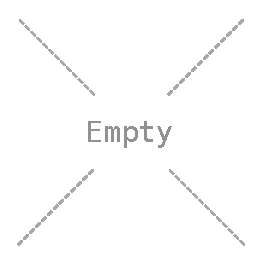
\includegraphics[height=\fgh]{empty.eps}
    \mycaption{fig:usecase-battery}{Battery saver use case}{Energy-Security
    Tradeoff vs Strict Energy Budget as discussed in Section \ref{??}. The graph
    shows median sequential write total energy use with respect to time with
    respect to time.}
\end{figure}
 \hsg{we should exlude ChaCha8 only, unless you have a
major point here}

% About: result
\figref{usecase-battery} shows the time versus energy used. At 0 seconds, we
begin writing. At 5 seconds, the ``battery saver'' event occurs, causing the
system to be underclocked. At 120 seconds, the system will die. If we blow past
our energy ceiling, the system will die. The figure shows two lines:
%
{\bf (1)} {\em Freestyle Balanced only}, that favors security even when backups
are paused;  the device dies before the I/Os complete.
%
{\bf (2)} {\em Freestyle Balanced $+$ ChaCha8}, that performs the switch when
the system enters the low power state. Our results show that, while the system
uses slightly more power in the short term, we stay within our energy budget and
finish before the devices dies.
%
When we get the device to a charger (not shown), the cloud backup is enabled
again and when the nuggets are read, \sys automatically converges them back to
Freestyle Balanced.

% About: overall result
On average, using forward switching resulted in a 3.3x total energy reduction
compared to exclusively using Freestyle Balanced, allowing us to remain within
our energy budget. \hsg{I don't see this 3.3x in the graph. Did you accidentally
label the lines incorrectly?}.  We note, however, that the energy savings is not
the point of this experiment. Rather, the lesson learned is that \sys enables
the system to move to the right point in the energy/security tradeoff space so
that the current task can still be accomplished before the battery is drained
and without compromising backup security at any point.


% ===============================
\subsection{End-of-Life Device Slowdown}\label{subsec:uc3}

Another usecase of forward switching is for offsetting the debilitating decline
in performance when storage devices such as SSDs reach end-of-life (EoL); due to
garbage collection and wear-leveling requirements of SSDs, as free space becomes
constrained, I/O performance drops precipitously~\cite{SSDEOL1}.  Let us suppose
in this case, the system running on the dying SSDs have a strict latency budget
(as long as meeting some minimum security requirements).  The strict latency
ceiling can be violated if the device latency increases.  If \sys is made aware
when the drive is in such a state, we can offset some of the performance loss by
switching the ciphers of high traffic nuggets to the fastest acceptable cipher
available using forward switching.

\def \fgh {1in}

\begin{figure}[t]
    \centering
    % {\begin{tikzpicture}[baseline]

    \pgfmathsetmacro{\ymax}{1.1} % set the maximum y value
    \pgfmathsetmacro{\ymaxbreak}{1.2} % set the y value at which overflow is drawn

    \begin{groupplot}[
        group style={
            group size=2 by 2,
            xlabels at=edge bottom,
            ylabels at=edge left,
            xticklabels at=edge bottom,
            yticklabels at=edge left,
            vertical sep=25pt,
            horizontal sep=15pt,
        },
        %axis x line*=bottom,
        scatter,
        point meta=explicit,
        scatter/classes={
            1={},
            2={dashed},
            3={mark=triangle*,red,mark size=2.5pt},
            4={mark=triangle*,orange,mark size=3pt},
            5={mark=square*,blue,mark size=2pt}
        },
        height=3.5cm,
        width=\linewidth/1.75,
        tick align=outside,
        tick pos=bottom, % make sure ticks only appear at the bottom and left axes
        title style={yshift=-1.5ex},
        tick style={ black },
        y tick label style={ /pgf/number format/fixed, /pgf/number format/precision=0 },
        grid style={ dotted, gray },
        %every node near coord/.append style={font=\tiny},
        %
        % magic to make the numbers appear above the overly long bars:
        % visualization depends on={rawy \as \rawy}, % save original y values
        % restrict y to domain*={ % now clip/restrict any y value to ymax
        %     \pgfkeysvalueof{/pgfplots/ymin}:\ymaxbreak
        % },
        % after end axis/.code={ % draw squiggly line indicating break
        %     \draw [semithick, white, decoration={snake,amplitude=0.1mm,segment length=0.75mm,post length=0.375mm}, decorate] (rel axis cs:0,1.01) -- (rel axis cs:1,1.01);
        % },
        % nodes near coords={\color{.!75!black}\pgfmathprintnumber\rawy}, % print the original y values (darkened in case they are too light)...
        % nodes near coords greater equal only=\ymax, % ... but ONLY if they are >= ymax
        % clip=false, % allow clip to protrude beyond ymax
        % Custom stuff to edit per template
        %
        xlabel={\footnotesize Security Score},
        xlabel near ticks,
        %xlabel shift={-1.5mm},
        xmin=0, xmax=4,
        xtick={ 0, 1, 2, 3, 4 },
        xticklabels={ 0,,, 3, \empty },
        %major x tick style=transparent,
        %enlarge x limits=0.2, % add some breathing room along the x axis's sides
        %
        ylabel={\footnotesize Latency (normalized)},
        ylabel near ticks,
        ylabel shift={-1.5mm},
        ymajorgrids=true,
        ymin=0, ymax=\ymax,
        ytick={ 0, 1, \ymax },
        yticklabels={ 0, 1, \empty },
        %yticklabels={ 0, 0.5, 1.5, 2 },
        % extra y ticks={1},
        % extra y tick style={grid=major, grid style={dashed, black}},
        % extra y tick label={\empty},
        %bar width=4.5pt, % change size of bars
        %
        legend cell align=center,
        legend style={ column sep=1ex },
        legend entries={%
            {\scriptsize Normal},
            {\scriptsize Delayed},
            {\scriptsize Choice Config (Normal)},
            {\scriptsize Bad Config (Delayed)},
            {\scriptsize Choice Config (Delayed)}
        },
        legend style={
            draw=none,
            legend columns=2,
            at={(1.0,1.25)},
            anchor=south,
        },
    ]
        \nextgroupplot[title={Sequential Reads}]
            \addplot [thick] table [
                meta=label,
                x=score,
                y=latency,
                discard if symbol not={iop}{r},
                discard if symbol not={delayed}{no},
                discard if symbol not={order}{seq},
                col sep=space,
            ] {data/usecase-eol-tradeoff.dat};
            \addplot [thick, dashed] table [
                meta=label,
                x=score,
                y=latency,
                discard if symbol not={iop}{r},
                discard if symbol not={delayed}{yes},
                discard if symbol not={order}{seq},
                col sep=space
            ] {data/usecase-eol-tradeoff.dat};
            \coordinate (c1) at (2.3, 0.8);
            \coordinate (c2) at (0.9, 0.96);
            \draw [dotted] (1.9, 0) -- (1.9, 1.1) node [left of=c1] {\tiny (security floor)};
            \draw [dotted] (0, 0.3) -- (4, 0.3) node [below of=c2] {\tiny (latency ceiling)};
        \nextgroupplot[legend to name={throwaway9}, title={Random Reads}]
            \addplot [thick] table [
                meta=label,
                x=score,
                y=latency,
                discard if symbol not={iop}{r},
                discard if symbol not={delayed}{no},
                discard if symbol not={order}{rnd},
                col sep=space
            ] {data/usecase-eol-tradeoff.dat};
            \addplot [thick, dashed] table [
                meta=label,
                x=score,
                y=latency,
                discard if symbol not={iop}{r},
                discard if symbol not={delayed}{yes},
                discard if symbol not={order}{rnd},
                col sep=space
            ] {data/usecase-eol-tradeoff.dat};
            \coordinate (c3) at (2.3, 0.8);
            \coordinate (c4) at (0.9, 0.96);
            \draw [dotted] (1.9, 0) -- (1.9, 1.1) node [left of=c3] {\tiny (security floor)};
            \draw [dotted] (0, 0.3) -- (4, 0.3) node [below of=c4] {\tiny (latency ceiling)};
        \nextgroupplot[legend to name={throwaway10}, title={Sequential Writes}]
            \addplot [thick] table [
                meta=label,
                x=score,
                y=latency,
                discard if symbol not={iop}{w},
                discard if symbol not={delayed}{no},
                discard if symbol not={order}{seq},
                col sep=space
            ] {data/usecase-eol-tradeoff.dat};
            \addplot [thick, dashed] table [
                meta=label,
                x=score,
                y=latency,
                discard if symbol not={iop}{w},
                discard if symbol not={delayed}{yes},
                discard if symbol not={order}{seq},
                col sep=space
            ] {data/usecase-eol-tradeoff.dat};
            \coordinate (c5) at (2.3, 0.8);
            \coordinate (c6) at (0.9, 0.96);
            \draw [dotted] (1.9, 0) -- (1.9, 1.1) node [left of=c5] {\tiny (security floor)};
            \draw [dotted] (0, 0.3) -- (4, 0.3) node [below of=c6] {\tiny (latency ceiling)};
        \nextgroupplot[legend to name={throwaway11}, title={Random Writes}]
            \addplot [thick] table [
                meta=label,
                x=score,
                y=latency,
                discard if symbol not={iop}{w},
                discard if symbol not={delayed}{no},
                discard if symbol not={order}{rnd},
                col sep=space
            ] {data/usecase-eol-tradeoff.dat};
            \addplot [thick, dashed] table [
                meta=label,
                x=score,
                y=latency,
                discard if symbol not={iop}{w},
                discard if symbol not={delayed}{yes},
                discard if symbol not={order}{rnd},
                col sep=space
            ] {data/usecase-eol-tradeoff.dat};
            \coordinate (c7) at (2.3, 0.8);
            \coordinate (c8) at (0.9, 0.96);
            \draw [dotted] (1.9, 0) -- (1.9, 1.1) node [left of=c7] {\tiny (security floor)};
            \draw [dotted] (0, 0.3) -- (4, 0.3) node [below of=c8] {\tiny (latency ceiling)};
    \end{groupplot}%
\end{tikzpicture}%
}
    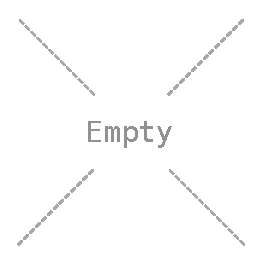
\includegraphics[height=\fgh]{empty.eps}
    \mycaption{fig:usecase-eol-tradeoff}{Device end-of-life use case}{SSD EoL Use
    Case: Latency-Security Tradeoff vs Goals.  Median sequential and random 40MB
    read and write performance comparison: baseline versus simulated faulty block
    device.}
\end{figure}


To show this, we begin by writing 10 40MB files per each cipher as a baseline.
\hsg{I don't understand ``per each cipher''} We then introduce a delay of $20ms$
simulating drive slowdown. \hsg{Where do you get ``20ms'' from?  that's such a
high latency. Any citation you can use here to back that up},
% --------------------------------------------------
\hsg{These sentences below are non informative. You should help reviewers walk
through the graph. I don't even understand what the x-axis in the Figure means.
The best way to describe a figure, is describe the x-axis and then y-axis, and
then pick two extreme points in the graph, and describe those points, what the
values mean, so that reviewers can really understand them. if reviewers
understand two extreme points, then they will undersstand the rest. Please redo
the sentences.}
% --------------------------------------------------
\sout{In \figref{usecase-eol-tradeoff}, we see the sequential and random read
and write performance of a 40MB workload when nuggets are encrypted exclusively
with our choice ciphers. While the latency ceiling and security floor have not
changed, we see increased latency in the delayed workloads. Our goal is to
remain under the latency ceiling while remaining above the security floor.
Thanks to Forward switching, accesses to highly trafficked areas of the drive
can remain performant even during drive end-of-life.}


% ================================================================
\subsection{Select Data Encryption}\label{subsec:uc2}

% About: background
This usecase illustrates utility of selective switching to achieve a performance
win---if only a small percentage of the data needs the strongest encryption,
then only a small percentage of the data should have that associated overhead,
while the rest can use a minimalist encryption. As mentioned before, this
feature requires users to annotate certain files with a special tag via file
system calls, which would then be stored in the inode.  Because the \sys layer
is file oblivious, every block I/O through the \sys layer will be labeled with
the corresponding cipher.

% About: setup
We begin by with 10 5MB and 4KB write-read operations to two \sys drive
instances: one using ChaCha8 and the other using Freestyle Strong.  They
represent two extreme where ChaCha8 is a low-latency cipher and Freestyle Strong
exhibits a very high overhead.  We then run another \sys instance with a 7:3
ratio where 30\% of the data considered highly sensitive uses Freestyle Strong.

\def \fgh {1in}

\begin{figure}[t]
    \centering
    %{\begin{tikzpicture}[baseline]

    \pgfmathsetmacro{\ymax}{20} % set the maximum y value
    \pgfmathsetmacro{\ymaxbreak}{20.1} % set the y value at which overflow is drawn

    \begin{axis}[
        %axis x line*=bottom,
        height=4cm,
        width=\linewidth,
        tick align=outside,
        tick pos=bottom, % make sure ticks only appear at the bottom and left axes
        tick style={ black },
        y tick label style={ /pgf/number format/fixed, /pgf/number format/precision=0 },
        grid style={ dotted, gray },
        every node near coord/.append style={font=\tiny},
        %
        % magic to make the numbers appear above the overly long bars:
        visualization depends on={rawy \as \rawy}, % save original y values
        restrict y to domain*={ % now clip/restrict any y value to ymax
            \pgfkeysvalueof{/pgfplots/ymin}:\ymaxbreak
        },
        after end axis/.code={ % draw squiggly line indicating break
            \draw [semithick, white, decoration={snake,amplitude=0.1mm,segment length=0.75mm,post length=0.375mm}, decorate] (rel axis cs:0,1.01) -- (rel axis cs:1,1.01);
        },
        nodes near coords={\color{.!75!black}\pgfmathprintnumber\rawy}, % print the original y values (darkened in case they are too light)...
        nodes near coords greater equal only=\ymax, % ... but ONLY if they are >= ymax
        clip=false, % allow clip to protrude beyond ymax
        % Custom stuff to edit per template
        %
        xlabel={\footnotesize Cipher Configuration},
        xlabel near ticks,
        xmin=C8, xmax=FS,
        xtick=data,
        symbolic x coords={C8,C8+FS,FS},
        enlarge x limits=0.2, % add some breathing room along the x axis's sides
        %major x tick style=transparent,
        %
        ylabel={\footnotesize Latency (s)},
        ylabel near ticks,
        ylabel shift={-1mm},
        ymajorgrids=true,
        ymin=0, ymax=\ymax,
        ybar, % value will shift bars
        ytick={ 0, 5, ..., \ymax },
        %yticklabels={ 0, 0.5, 1.5, 2 },
        % extra y ticks={1},
        % extra y tick style={grid=major, grid style={dashed, black}},
        % extra y tick label={\empty},
        %bar width=4.5pt, % change size of bars
        %
        legend cell align=center,
        legend style={ column sep=1ex },
        legend entries={
            {\scriptsize 4K/reads},
            {\scriptsize 4K/writes},
            {\scriptsize 5M/reads},
            {\scriptsize 5M/writes},
        },
        legend style={
            draw=none,
            legend columns=2,
            at={(0.5,1.02)},
            anchor=south,
        },
    ]
        \addplot[fill=orangeDark, every node near coord/.append style={color=orangeDark}]
        table[x=conf, y=latr-4k, col sep=space] {data/usecase-vsr-tradeoff.dat};
        \addplot[fill=orangeDark, postaction={pattern=north east lines}, every node near coord/.append style={color=purpleDark}]
        table[x=conf, y=latw-4k, col sep=space] {data/usecase-vsr-tradeoff.dat};
        \addplot[fill=purpleDark, every node near coord/.append style={color=orangeDark}]
        table[x=conf, y=latr-5m, col sep=space] {data/usecase-vsr-tradeoff.dat};
        \addplot[fill=purpleDark, postaction={pattern=north east lines}, every node near coord/.append style={color=purpleDark}]
        table[x=conf, y=latw-5m, col sep=space] {data/usecase-vsr-tradeoff.dat};
    \end{axis}%
\end{tikzpicture}%
}
    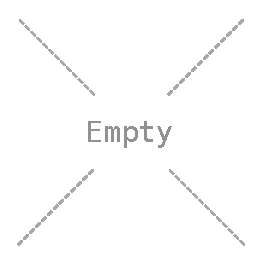
\includegraphics[height=\fgh]{empty.eps}
    \mycaption{fig:usecase-vsr-bar}{Selective file/region usecase}{VSR Use Case:
    ChaCha8 vs Freestyle Strong Sequential 4KB, 5MB Performance. The graph shows
    median sequential read and write performance comparison of 4KB, 5MB I/O with
    7-to-3 ratio, ChaCha8 vs Freestyle Strong (respectively).}
\end{figure}


% About: outcome
The left-side and right-side bars in \figref{usecase-vsr-bar} show the two
extremes; ChaCha8 exhibits a low latency, consistently less than 1 second across
the workloads, while Freestyle Strong exhibits 5 to 20 second latency depending
on the workload.  The selective switching (middle bars) shows a reduction of
3.1x to 4.8x for read latency and 1.6x to 2.8x for write latency, all without
compromising the security needs of the most sensitive data.  Thus, selective
switching keeps our sensitive data at the mandated security level while keeping
the performance (and also battery life) benefits of using a fast cipher for the
majority of I/O operations.


% ===============================
\subsection{No-Downtime Encryption Upgrade}\label{subsec:uc4}

\def \fgh {1in}

\begin{figure}[t]
    \centering
    %{\begin{tikzpicture}[baseline]

    \pgfmathsetmacro{\ymax}{1.1} % set the maximum y value
    \pgfmathsetmacro{\ymaxbreak}{1.2} % set the y value at which overflow is drawn

    \begin{groupplot}[
        group style={
            group size=2 by 2,
            xlabels at=edge bottom,
            ylabels at=edge left,
            xticklabels at=edge bottom,
            yticklabels at=edge left,
            vertical sep=25pt,
            horizontal sep=15pt,
        },
        %axis x line*=bottom,
        scatter,
        point meta=explicit,
        scatter/classes={
            1={},
            2={dashed},
            3={mark=triangle*,red,mark size=2.5pt},
            4={mark=triangle*,orange,mark size=3pt},
            5={mark=square*,blue,mark size=2pt}
        },
        height=3.5cm,
        width=\linewidth/1.75,
        tick align=outside,
        tick pos=bottom, % make sure ticks only appear at the bottom and left axes
        title style={yshift=-1.5ex},
        tick style={ black },
        y tick label style={ /pgf/number format/fixed, /pgf/number format/precision=0 },
        grid style={ dotted, gray },
        %every node near coord/.append style={font=\tiny},
        %
        % magic to make the numbers appear above the overly long bars:
        % visualization depends on={rawy \as \rawy}, % save original y values
        % restrict y to domain*={ % now clip/restrict any y value to ymax
        %     \pgfkeysvalueof{/pgfplots/ymin}:\ymaxbreak
        % },
        % after end axis/.code={ % draw squiggly line indicating break
        %     \draw [semithick, white, decoration={snake,amplitude=0.1mm,segment length=0.75mm,post length=0.375mm}, decorate] (rel axis cs:0,1.01) -- (rel axis cs:1,1.01);
        % },
        % nodes near coords={\color{.!75!black}\pgfmathprintnumber\rawy}, % print the original y values (darkened in case they are too light)...
        % nodes near coords greater equal only=\ymax, % ... but ONLY if they are >= ymax
        % clip=false, % allow clip to protrude beyond ymax
        % Custom stuff to edit per template
        %
        xlabel={\footnotesize Security Score},
        xlabel near ticks,
        %xlabel shift={-1.5mm},
        xmin=0, xmax=4,
        xtick={ 0, 1, 2, 3, 4 },
        xticklabels={ 0,,, 3, \empty },
        %major x tick style=transparent,
        %enlarge x limits=0.2, % add some breathing room along the x axis's sides
        %
        ylabel={\footnotesize Latency (normalized)},
        ylabel near ticks,
        ylabel shift={-1.5mm},
        ymajorgrids=true,
        ymin=0, ymax=\ymax,
        ytick={ 0, 1, \ymax },
        yticklabels={ 0, 1, \empty },
        %yticklabels={ 0, 0.5, 1.5, 2 },
        % extra y ticks={1},
        % extra y tick style={grid=major, grid style={dashed, black}},
        % extra y tick label={\empty},
        %bar width=4.5pt, % change size of bars
        %
        legend cell align=center,
        legend style={ column sep=1ex },
        legend entries={%
            {\scriptsize Normal},
            {\scriptsize Delayed},
            {\scriptsize Choice Config (Normal)},
            {\scriptsize Bad Config (Delayed)},
            {\scriptsize Choice Config (Delayed)}
        },
        legend style={
            draw=none,
            legend columns=2,
            at={(1.0,1.25)},
            anchor=south,
        },
    ]
        \nextgroupplot[title={Sequential Reads}]
            \addplot [thick] table [
                meta=label,
                x=score,
                y=latency,
                discard if symbol not={iop}{r},
                discard if symbol not={delayed}{no},
                discard if symbol not={order}{seq},
                col sep=space,
            ] {data/usecase-eol-tradeoff.dat};
            \addplot [thick, dashed] table [
                meta=label,
                x=score,
                y=latency,
                discard if symbol not={iop}{r},
                discard if symbol not={delayed}{yes},
                discard if symbol not={order}{seq},
                col sep=space
            ] {data/usecase-eol-tradeoff.dat};
            \coordinate (c1) at (2.3, 0.8);
            \coordinate (c2) at (0.9, 0.96);
            \draw [dotted] (1.9, 0) -- (1.9, 1.1) node [left of=c1] {\tiny (security floor)};
            \draw [dotted] (0, 0.3) -- (4, 0.3) node [below of=c2] {\tiny (latency ceiling)};
        \nextgroupplot[legend to name={throwaway9}, title={Random Reads}]
            \addplot [thick] table [
                meta=label,
                x=score,
                y=latency,
                discard if symbol not={iop}{r},
                discard if symbol not={delayed}{no},
                discard if symbol not={order}{rnd},
                col sep=space
            ] {data/usecase-eol-tradeoff.dat};
            \addplot [thick, dashed] table [
                meta=label,
                x=score,
                y=latency,
                discard if symbol not={iop}{r},
                discard if symbol not={delayed}{yes},
                discard if symbol not={order}{rnd},
                col sep=space
            ] {data/usecase-eol-tradeoff.dat};
            \coordinate (c3) at (2.3, 0.8);
            \coordinate (c4) at (0.9, 0.96);
            \draw [dotted] (1.9, 0) -- (1.9, 1.1) node [left of=c3] {\tiny (security floor)};
            \draw [dotted] (0, 0.3) -- (4, 0.3) node [below of=c4] {\tiny (latency ceiling)};
        \nextgroupplot[legend to name={throwaway10}, title={Sequential Writes}]
            \addplot [thick] table [
                meta=label,
                x=score,
                y=latency,
                discard if symbol not={iop}{w},
                discard if symbol not={delayed}{no},
                discard if symbol not={order}{seq},
                col sep=space
            ] {data/usecase-eol-tradeoff.dat};
            \addplot [thick, dashed] table [
                meta=label,
                x=score,
                y=latency,
                discard if symbol not={iop}{w},
                discard if symbol not={delayed}{yes},
                discard if symbol not={order}{seq},
                col sep=space
            ] {data/usecase-eol-tradeoff.dat};
            \coordinate (c5) at (2.3, 0.8);
            \coordinate (c6) at (0.9, 0.96);
            \draw [dotted] (1.9, 0) -- (1.9, 1.1) node [left of=c5] {\tiny (security floor)};
            \draw [dotted] (0, 0.3) -- (4, 0.3) node [below of=c6] {\tiny (latency ceiling)};
        \nextgroupplot[legend to name={throwaway11}, title={Random Writes}]
            \addplot [thick] table [
                meta=label,
                x=score,
                y=latency,
                discard if symbol not={iop}{w},
                discard if symbol not={delayed}{no},
                discard if symbol not={order}{rnd},
                col sep=space
            ] {data/usecase-eol-tradeoff.dat};
            \addplot [thick, dashed] table [
                meta=label,
                x=score,
                y=latency,
                discard if symbol not={iop}{w},
                discard if symbol not={delayed}{yes},
                discard if symbol not={order}{rnd},
                col sep=space
            ] {data/usecase-eol-tradeoff.dat};
            \coordinate (c7) at (2.3, 0.8);
            \coordinate (c8) at (0.9, 0.96);
            \draw [dotted] (1.9, 0) -- (1.9, 1.1) node [left of=c7] {\tiny (security floor)};
            \draw [dotted] (0, 0.3) -- (4, 0.3) node [below of=c8] {\tiny (latency ceiling)};
    \end{groupplot}%
\end{tikzpicture}%
}
    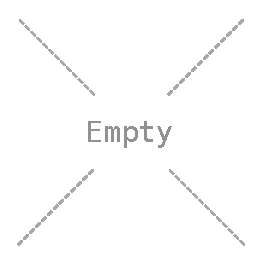
\includegraphics[height=\fgh]{empty.eps}
    \mycaption{fig:usecase4}{Fix-me-todo}{\TODO{This.}}
\end{figure}


In \figref{usecase4} \TODO{finish sentence}. \hsg{we must have a short case
study here. Otherwise no point of talking about mirrored switch}.
